% This LaTeX document needs to be compiled with XeLaTeX.
\documentclass[10pt]{article}
\usepackage[utf8]{inputenc}
\usepackage{ucharclasses}
\usepackage{graphicx}
\usepackage[export]{adjustbox}
\graphicspath{ {./images/} }
\usepackage{amsmath}
\usepackage{amsfonts}
\usepackage{amssymb}
\usepackage[version=4]{mhchem}
\usepackage{stmaryrd}
\usepackage{hyperref}
\hypersetup{colorlinks=true, linkcolor=blue, filecolor=magenta, urlcolor=cyan,}
\urlstyle{same}
\usepackage{multirow}
\usepackage[fallback]{xeCJK}
\usepackage{polyglossia}
\usepackage{fontspec}
\setCJKmainfont{Noto Serif CJK KR}

\setmainlanguage{polish}
\setotherlanguages{bengali}
\newfontfamily\bengalifont{Noto Serif Bengali}
\newfontfamily\lgcfont{CMU Serif}
\setDefaultTransitions{\lgcfont}{}
\setTransitionsFor{Bengali}{\bengalifont}{\lgcfont}

\title{KOD }

\author{}
\date{}


\newcommand\Varangle{\mathop{{<\!\!\!\!\!\text{\small)}}\:}\nolimits}

\begin{document}
\maketitle
IMIĘ I NAZWISKO *\\
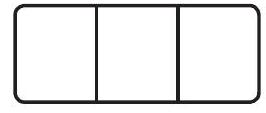
\includegraphics[max width=\textwidth, center]{2024_11_21_dd21f7544b65bcf1b3c7g-01}\\
\(\square\)

\begin{itemize}
  \item nieobowiązkowe
\end{itemize}

\section*{PRÓBNY EGZAMIN MATURALNY Z NOWĄ ERĄ MATEMATYKA - POZIOM PODSTAWOWY}
\section*{Instrukcja dla zdającego}
\begin{enumerate}
  \item Sprawdź, czy arkusz egzaminacyjny zawiera 22 strony (zadania 1-32) i kartę odpowiedzi. Ewentualny brak stron zgłoś nauczycielowi nadzorującemu egzamin.
  \item Rozwiązania zadań i odpowiedzi zapisz w miejscu na to przeznaczonym.
  \item Pamiętaj, że pominięcie argumentacji lub istotnych obliczeń w rozwiązaniu zadań otwartych może spowodować, że za to rozwiązanie nie otrzymasz pełnej liczby punktów.
  \item Pisz czytelnie. Używaj długopisu/pióra tylko z czarnym tuszem/atramentem.
  \item Nie używaj korektora, a błędne zapisy wyraźnie przekreśl.
  \item Pamiętaj, że zapisy w brudnopisie nie będą oceniane.
  \item Podczas egzaminu możesz korzystać z zestawu wzorów matematycznych, cyrkla i linijki oraz kalkulatora prostego.
  \item Na tej stronie i na karcie odpowiedzi wpisz swój kod oraz imię i nazwisko.
  \item Odpowiedzi do zadań zamkniętych przenieś na kartę odpowiedzi, zaznaczając je w części karty przeznaczonej dla zdającego.
  \item Nie wpisuj żadnych znaków w części przeznaczonej dla osoby sprawdzającej.\\
\(\square\) dysleksja
\end{enumerate}

STYCZEŃ 2017

Czas pracy:\\
170 minut

Liczba punktów\\
do uzyskania: 50

W zadaniach od 1. do 23. wybierz i zaznacz na karcie odpowiedzi poprawną odpowiedź.\\
Zadanie 1. (0-1)\\
Liczba \(\frac{6}{\sqrt[3]{27}}\) jest równa\\
A. \(6 \cdot 27^{\frac{1}{3}}\)\\
B. \(\frac{2}{3}\)\\
C. \(\frac{6}{3^{3}}\)\\
D. 2

Zadanie 2. (0-1)\\
Liczba \(\sqrt{(1-2 \sqrt{2})^{2}}\) jest równa\\
A. \(1-2 \sqrt{2}\)\\
B. \(2 \sqrt{2}-1\)\\
C. \(\sqrt{9+4 \sqrt{2}}\)\\
D. \(\sqrt{7}\)

\section*{Zadanie 3. (0-1)}
Nowy samochód kosztował 80 tys. zł. Po każdym roku użytkowania jego wartość spadała o 15\% w stosunku do wartości z roku poprzedniego. Po trzech latach od zakupu jego wartość była równa\\
A. \(36000 \mathrm{zł}\)\\
B. \(44000 \mathrm{zł}\)\\
C. \(49130 \mathrm{zł}\)\\
D. \(57800 \mathrm{zł}\)

\section*{Zadanie 4. (0-1)}
Pan Adam wpłacał na rzecz pewnego stowarzyszenia 2\% swoich stałych miesięcznych dochodów. Od ostatniego miesiąca wpłata wzrosła do \(3 \%\) jego dochodów. O ile procent zwiększyła się kwota wpłacana przez pana Adama?\\
A. o \(1 \%\)\\
B. \(\mathrm{o} 30 \%\)\\
C. o \(50 \%\)\\
D. \(\mathrm{o} 150 \%\)

\section*{Zadanie 5. (0-1)}
Na rysunku przedstawiono wykres funkcji \(y=h(x)\).\\
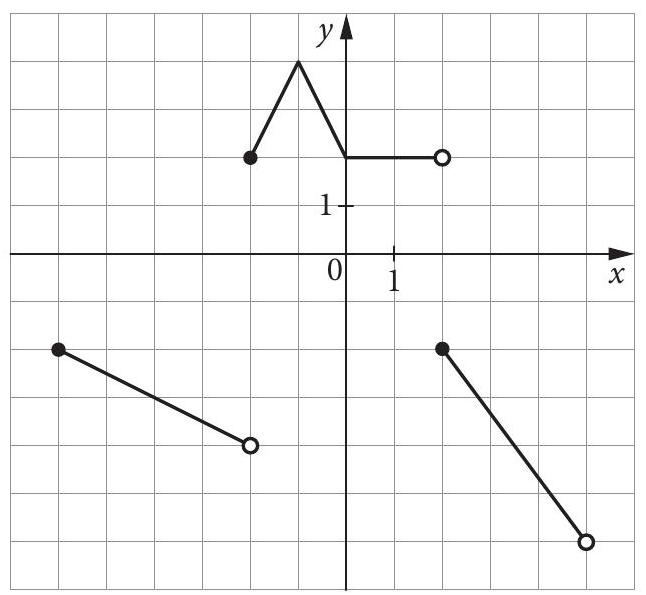
\includegraphics[max width=\textwidth, center]{2024_11_21_dd21f7544b65bcf1b3c7g-02}

Dziedziną funkcji \(h\) jest przedział\\
A. \(\langle-2,2)\)\\
B. \(\langle-6,5)\)\\
C. \((-6,5)\)\\
D. \((-6,4)\)

\section*{Zadanie 6. (0-1)}
Funkcja \(f\) każdej liczbie naturalnej przyporządkowuje resztę z dzielenia tej liczby przez 3. Zbiór wartości tej funkcji to\\
A. \(\{0,1\}\)\\
B. \(\{0,2\}\)\\
C. \(\{1,2\}\)\\
D. \(\{0,1,2\}\)\\

\includegraphics[max width=\textwidth, center]{2024_11_21_dd21f7544b65bcf1b3c7g-03}

\section*{Zadanie 7. (0-1)}
Wykres funkcji \(f(x)=\frac{4}{x}\), określonej dla wszystkich liczb rzeczywistych różnych od 0 , przesunięto wzdłuż osi Oy o 4 jednostki w górę. Otrzymany wykres można opisać wzorem\\
A. \(g(x)=\frac{4}{x}+4\)\\
B. \(g(x)=\frac{4}{x}-4\)\\
C. \(g(x)=\frac{4}{x+4}\)\\
D. \(g(x)=\frac{4}{x-4}\)

\section*{Zadanie 8. (0-1)}
Funkcja wykładnicza \(f(x)=3^{x}\) przyjmuje wartość 4 dla\\
A. \(2 \log 2\)\\
B. \(\log _{3} 12\)\\
C. \(\log _{4} 3\)\\
D. \(2 \log _{3} 2\)

Zadanie 9. (0-1)\\
Funkcja liniowa \(f(x)=a x+b\) jest malejąca i ma ujemne miejsce zerowe. Dla takiej funkcji prawdziwa jest nierówność\\
A. \(a+b>0\)\\
B. \(a+b<0\)\\
C. \(a b=0\)\\
D. \(a b<0\)

\section*{Zadanie 10. (0-1)}
Na rysunku przedstawiony jest fragment wykresu pewnej funkcji kwadratowej postaci \(f(x)=a x^{2}+c\).\\
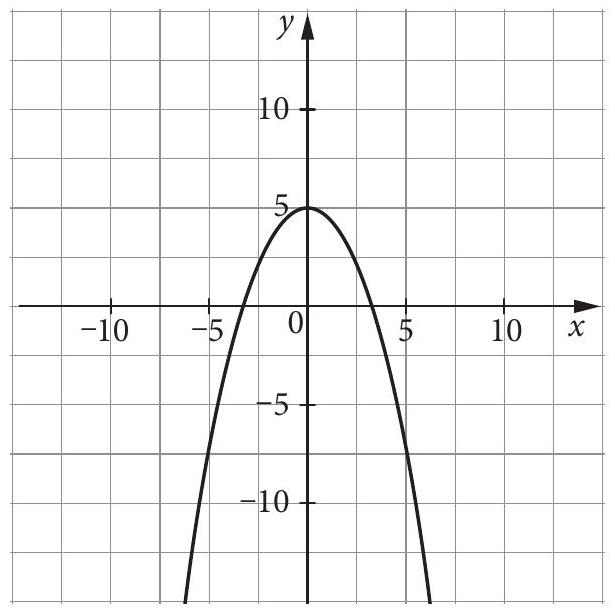
\includegraphics[max width=\textwidth, center]{2024_11_21_dd21f7544b65bcf1b3c7g-04}

Jakie znaki mają współczynniki \(a\) i \(c\) ?\\
A. \(a>0, c<0\)\\
B. \(a<0, c>0\)\\
C. \(a>0, c>0\)\\
D. \(a<0, c<0\)

\section*{Zadanie 11. (0-1)}
Wskaż liczby, które należy wpisać do tabeli, aby wielkości \(x\) i \(y\) były odwrotnie proporcjonalne.

\begin{center}
\begin{tabular}{|l|l|c|c|}
\hline
\(x\) &  & 2 & 0,5 \\
\hline
\(y\) & 16 & 24 &  \\
\hline
\end{tabular}
\end{center}

A. \(x=6, y=22,5\)\\
B. \(x=\frac{4}{3}, y=6\)\\
C. \(x=3, y=96\)\\
D. \(x=4, y=1\)

Więcej arkuszy znajdziesz na stronie: \href{http://arkusze.pl}{arkusze.pl}\\

\includegraphics[max width=\textwidth, center]{2024_11_21_dd21f7544b65bcf1b3c7g-05}

Zadanie 12. (0-1)\\
Ciąg \(\left(a_{n}\right)\) jest określony wzorem \(a_{n}=(-1)^{n} \cdot \frac{n}{n+1}\) dla \(n \geqslant 1\). Iloczyn \(a_{1} \cdot a_{2} \cdot a_{3}\) jest równy\\
A. \(-\frac{1}{2}\)\\
B. \(-\frac{1}{4}\)\\
C. 0\\
D. \(\frac{1}{4}\)

\section*{Zadanie 13. (0-1)}
Ciąg \(\left(a_{n}\right)\) jest określony wzorem \(a_{n}=4(n+1)(n-10)\) dla \(n \geqslant 1\). Ile wyrazów ujemnych ma ten ciąg?\\
A. 9\\
B. 10\\
C. 11\\
D. 12

\section*{Zadanie 14. (0-1)}
Ciąg \((a, b, c)\) jest ciągiem arytmetycznym o różnicy 2 , a ciąg \((d, e, f)\) jest ciągiem arytmetycznym o różnicy 4. Różnica ciągu arytmetycznego ( \(a+d, b+e, c+f\) ) wynosi\\
A. -6\\
B. -2\\
C. 2\\
D. 6

\section*{Zadanie 15. (0-1)}
Wartość wyrażenia \(\frac{\cos ^{2} 30^{\circ}+\cos ^{2} 60^{\circ}}{\cos 45^{\circ}}\) jest równa\\
A. \(\frac{3}{4}\)\\
B. 1\\
C. \(\sqrt{2}\)\\
D. \(\frac{\sqrt{3}}{2}\)

\section*{Zadanie 16. (0-1)}
Odcinek \(A B\) jest średnicą koła (rysunek obok). Na jednym z łuków \(A B\) zaznaczono punkty \(C, D\) i \(E\) różne od \(A\) i \(B\). W ten sposób powstały łuki \(A C, C D, D E, E B\), których długości są w stosunku 1:1:2:4. Miary kątów \(A C B, A D B\) i \(A E B\) spełniają zależności\\
A. \(|\Varangle A C B|<|\Varangle A D B|<|\Varangle A E B|\)\\
B. \(|\Varangle A C B|=|\Varangle A D B|=|\Varangle A E B|\)\\
C. \(|\Varangle A C B|=|\Varangle A D B|<|\Varangle A E B|\)\\
D. \(|\Varangle A C B|<|\Varangle A D B|=|\Varangle A E B|\)\\
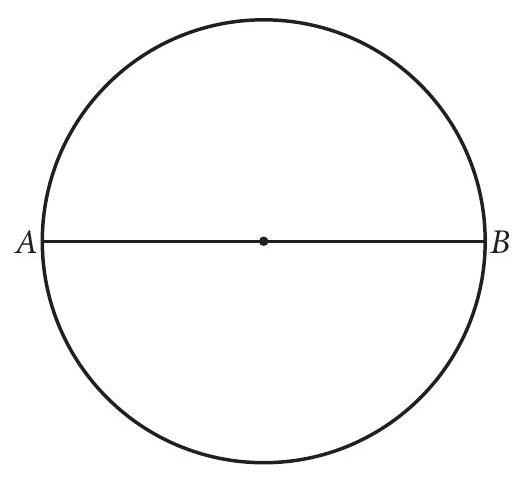
\includegraphics[max width=\textwidth, center]{2024_11_21_dd21f7544b65bcf1b3c7g-06}

\section*{Zadanie 17. (0-1)}
Pole rombu o boku długości \(6 \sqrt{3}\) i kącie rozwartym \(150^{\circ}\) jest równe\\
A. 27\\
B. \(27 \sqrt{3}\)\\
C. 54\\
D. \(54 \sqrt{3}\)

\section*{Zadanie 18. (0-1)}
Punkt \(A=(-1,3)\) jest wierzchołkiem trójkąta równoramiennego \(A B C\) o podstawie \(A B\). Punkt \(D=(5,-4)\) jest spodkiem wysokości \(C D\) tego trójkąta. Współrzędne wierzchołka \(B\) są równe\\
A. \((11,-11)\)\\
B. \((-11,11)\)\\
C. \((-7,10)\)\\
D. \((7,-10)\)

Więcej arkuszy znajdziesz na stronie: \href{http://arkusze.pl}{arkusze.pl}\\

\includegraphics[max width=\textwidth, center]{2024_11_21_dd21f7544b65bcf1b3c7g-07}

\section*{Zadanie 19. (0-1)}
Siatka ostrosłupa prawidłowego czworokątnego składa się z kwadratu i czterech trójkątów (rysunek obok). Pole każdej z wymienionych figur jest równe 4. Długość krawędzi bocznej tego ostrosłupa jest równa\\
A. \(\sqrt{5}\)\\
B. \(2 \sqrt{5}\)\\
C. \(\sqrt{17}\)\\
D. \(2 \sqrt{17}\)\\
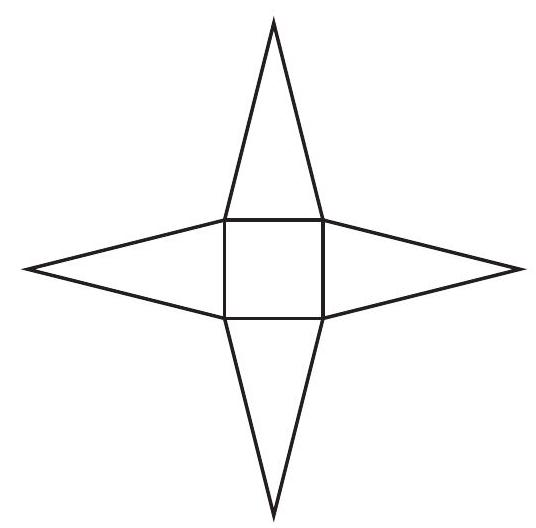
\includegraphics[max width=\textwidth, center]{2024_11_21_dd21f7544b65bcf1b3c7g-08(1)}

\section*{Zadanie 20. (0-1)}
Objętość stożka ściętego (rysunek obok) dana jest wzorem \(V=\frac{1}{3} \pi H\left(r^{2}+r R+R^{2}\right)\), gdzie \(H\) jest wysokością bryły, a \(r\) i \(R\) są promieniami jej podstaw.\\
Dane są: \(V=52 \pi, r=2, R=6\). Wysokość bryły jest równa\\
A. \(\frac{13}{7}\)\\
B. \(\frac{39}{7}\)\\
C. 1\\
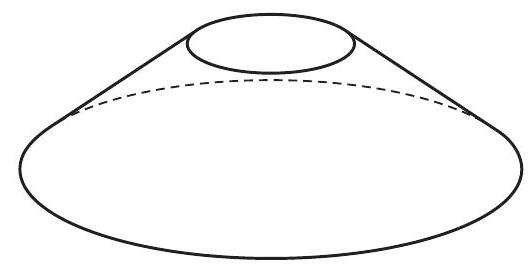
\includegraphics[max width=\textwidth, center]{2024_11_21_dd21f7544b65bcf1b3c7g-08}

Zadanie 21. (0-1)\\
Czterocyfrowy kod składa się z dwóch cyfr 0 i dwóch różnych cyfr wybranych spośród: 1, 2, 3, 4, 5 . Oto dwa przykładowe kody: 0250, 1003. Ile kodów spełnia opisane warunki?\\
A. 20\\
B. 80\\
C. 120\\
D. 150

\section*{Zadanie 22. (0-1)}
W tabeli podano oceny z matematyki pewnego ucznia.

\begin{center}
\begin{tabular}{|l|c|c|}
\hline
Kategoria & Waga oceny & Oceny \\
\hline
Odpowiedź ustna & 1 & 5,1 \\
\hline
Zadanie domowe & 2 & 4 \\
\hline
Sprawdzian & 2 & 2 \\
\hline
Zadanie klasowe & 3 & 4,3 \\
\hline
Aktywność & 1 & 5 \\
\hline
\end{tabular}
\end{center}

Średnia ważona tego zestawu danych w zaokrągleniu do dwóch miejsc po przecinku jest równa\\
A. 2,67\\
B. 3,38\\
C. 3,43\\
D. 4,89

\section*{Zadanie 23. (0-1)}
W urnie było 9 kul, trzy z nich były koloru białego. Do urny dołożono jeszcze cztery kule białe. Po tej zmianie prawdopodobieństwo wylosowania kuli białej jest równe\\
A. \(\frac{3}{13}\)\\
B. \(\frac{4}{13}\)\\
C. \(\frac{7}{13}\)\\
D. \(\frac{9}{13}\)

Więcej arkuszy znajdziesz na stronie: \href{http://arkusze.pl}{arkusze.pl}\\

\includegraphics[max width=\textwidth, center]{2024_11_21_dd21f7544b65bcf1b3c7g-09}

Zadanie 24. (0-2)\\
Zbiór wartości funkcji \(f(x)=(2 a+b) x^{2}+(a+b-4) x-7\) określonej dla wszystkich liczb\\
rzeczywistych \(x\) jest jednoelementowy. Wyznacz \(a\) i \(b\).\\

\includegraphics[max width=\textwidth, center]{2024_11_21_dd21f7544b65bcf1b3c7g-10}

Odpowiedź:

Zadanie 25. (0-2)\\
Dana jest funkcja \(f\) określona wzorem \(f(x)=(a+1)(x-2)^{2}(x+1)\) dla wszystkich liczb rzeczywistych \(x\). Dla jakich wartości \(a\) spełniona jest nierówność \(f(0) \cdot f(1) \leqslant 16\) ?\\

\includegraphics[max width=\textwidth, center]{2024_11_21_dd21f7544b65bcf1b3c7g-11}

Odpowiedź:

\begin{center}
\begin{tabular}{|c|l|c|c|}
\hline
\multirow{3}{*}{\begin{tabular}{c}
Wypełnia \\
sprawdzający \\
\end{tabular}} & Nr zadania & 24 & 25 \\
\cline { 2 - 4 }
 & Maks. liczba pkt & 2 & 2 \\
\cline { 2 - 4 }
 & Uzyskana liczba pkt &  &  \\
\hline
\end{tabular}
\end{center}

Zadanie 26. (0-2)\\
Do kwadratu różnicy dwóch dowolnych liczb parzystych dodano różnicę kwadratów tych liczb. Udowodnij, że otrzymana liczba jest podzielna przez 8.\\

\includegraphics[max width=\textwidth, center]{2024_11_21_dd21f7544b65bcf1b3c7g-12}

Zadanie 27. (0-2)\\
Dany jest trójkąt o bokach długości \(a, b\) i \(c\). Uzasadnij, że suma obwodów kół o średnicach \(a\) i \(b\) jest większa od obwodu koła o średnicy \(c\).\\

\includegraphics[max width=\textwidth, center]{2024_11_21_dd21f7544b65bcf1b3c7g-13}

\begin{center}
\begin{tabular}{|c|l|c|c|}
\hline
\multirow{3}{*}{\begin{tabular}{c}
Wypełnia \\
sprawdzający \\
\end{tabular}} & Nr zadania & 26 & 27 \\
\cline { 2 - 4 }
 & Maks. liczba pkt & 2 & 2 \\
\cline { 2 - 4 }
 & Uzyskana liczba pkt &  &  \\
\hline
\end{tabular}
\end{center}

\section*{Zadanie 28. (0-2)}
Na trójkącie opisano okrąg. Wierzchołki trójkąta podzieliły ten okrąg na łuki, których długości pozostają w stosunku \(10: 6: 4\). Odczytaj z tablic i zapisz przybliżoną wartość cosinusa najmniejszego kąta tego trójkąta.

\begin{center}
\begin{tabular}{|c|c|c|c|c|c|c|c|c|c|c|c|c|c|c|c|c|c|c|c|c|c|c|c|c|c|c|c|c|c|}
\hline
 &  &  &  &  &  &  &  &  &  &  &  &  &  &  &  &  &  &  &  &  &  &  &  &  &  &  &  &  &  \\
\hline
 &  &  &  &  &  &  &  &  &  &  &  &  &  &  &  &  &  &  &  &  &  &  &  &  &  &  &  &  &  \\
\hline
 &  &  &  &  &  &  &  &  &  &  &  &  &  &  &  &  &  &  &  &  &  &  &  &  &  &  &  &  &  \\
\hline
 &  &  &  &  &  &  &  &  &  &  &  &  &  &  &  &  &  &  &  &  &  &  &  &  &  &  &  &  &  \\
\hline
 &  &  &  &  &  &  &  &  &  &  &  &  &  &  &  &  &  &  &  &  &  &  &  &  &  &  &  &  &  \\
\hline
 &  &  &  &  &  &  &  &  &  &  &  &  &  &  &  &  &  &  &  &  &  &  &  &  &  &  &  &  &  \\
\hline
 &  &  &  &  &  &  &  &  &  &  &  &  &  &  &  &  &  &  &  &  &  &  &  &  &  &  &  &  &  \\
\hline
 &  &  &  &  &  &  &  &  &  &  &  &  &  &  &  &  &  &  &  &  &  &  &  &  &  &  &  &  &  \\
\hline
 &  &  &  &  &  &  &  &  &  &  &  &  &  &  &  &  &  &  &  &  &  &  &  &  &  &  &  &  &  \\
\hline
 &  &  &  &  &  &  &  &  &  &  &  &  &  &  &  &  &  &  &  &  &  &  &  &  &  &  &  &  &  \\
\hline
 &  &  &  &  &  &  &  &  &  &  &  &  &  &  &  &  &  &  &  &  &  &  &  &  &  &  &  &  &  \\
\hline
 &  &  &  &  &  &  &  &  &  &  &  &  &  &  &  &  &  &  &  &  &  &  &  &  &  &  &  &  &  \\
\hline
 &  &  &  &  &  &  &  &  &  &  &  &  &  &  &  &  &  &  &  &  &  &  &  &  &  &  &  &  &  \\
\hline
 &  &  &  &  &  &  &  &  &  &  &  &  &  &  &  &  &  &  &  &  &  &  &  &  &  &  &  &  &  \\
\hline
 &  &  &  &  &  &  &  &  &  &  &  &  &  &  &  &  &  &  &  &  &  &  &  &  &  &  &  &  &  \\
\hline
 &  &  &  &  &  &  &  &  &  &  &  &  &  &  &  &  &  &  &  &  &  &  &  &  &  &  &  &  &  \\
\hline
 &  &  &  &  &  &  &  &  &  &  &  &  &  &  &  &  &  &  &  &  &  &  &  &  &  &  &  &  &  \\
\hline
 &  &  &  &  &  &  &  &  &  &  &  &  &  &  &  &  &  &  &  &  &  &  &  &  &  &  &  &  &  \\
\hline
 &  &  &  &  &  &  &  &  &  &  &  &  &  &  &  &  &  &  &  &  &  &  &  &  &  &  &  &  &  \\
\hline
 &  &  &  &  &  &  &  &  &  &  &  &  &  &  &  &  &  &  &  &  &  &  &  &  &  &  &  &  &  \\
\hline
 &  &  &  &  &  &  &  &  &  &  &  &  &  &  &  &  &  &  &  &  &  &  &  &  &  &  &  &  &  \\
\hline
 &  &  &  &  &  &  &  &  &  &  &  &  &  &  &  &  &  &  &  &  &  &  &  &  &  &  &  &  &  \\
\hline
 &  &  &  &  &  &  &  &  &  &  &  &  &  &  &  &  &  &  &  &  &  &  &  &  &  &  &  &  &  \\
\hline
 &  &  &  &  &  &  &  &  &  &  &  &  &  &  &  &  &  &  &  &  &  &  &  &  &  &  &  &  &  \\
\hline
 &  &  &  &  &  &  &  &  &  &  &  &  &  &  &  &  &  &  &  &  &  &  &  &  &  &  &  &  &  \\
\hline

\includegraphics[max width=\textwidth]{2024_11_21_dd21f7544b65bcf1b3c7g-14(1)}
 &  &  &  &  &  &  &  &  &  &  &  &  &  &  &  &  &  &  &  &  &  &  &  &  &  &  &  &  &  \\
\hline

\includegraphics[max width=\textwidth]{2024_11_21_dd21f7544b65bcf1b3c7g-14}
 &  &  &  &  &  &  &  &  &  &  &  &  &  &  &  &  &  &  &  &  &  &  &  &  &  &  &  &  &  \\
\hline
 &  &  &  &  &  &  &  &  &  &  &  &  &  &  &  &  &  &  &  &  &  &  &  &  &  &  &  &  &  \\
\hline
 &  &  &  &  &  &  &  &  &  &  &  &  &  &  &  &  &  &  &  &  &  &  &  &  &  &  &  &  &  \\
\hline
 &  &  &  &  &  &  &  &  &  &  &  &  &  &  &  &  &  &  &  &  &  &  &  &  &  &  &  &  &  \\
\hline
 &  &  &  &  &  &  &  &  &  &  &  &  &  &  &  &  &  &  &  &  &  &  &  &  &  &  &  &  &  \\
\hline
 &  &  &  &  &  &  &  &  &  &  &  &  &  &  &  &  &  &  &  &  &  &  &  &  &  &  &  &  &  \\
\hline
 &  &  &  &  &  &  &  &  &  &  &  &  &  &  &  &  &  &  &  &  &  &  &  &  &  &  &  &  &  \\
\hline
 &  &  &  &  &  &  &  &  &  &  &  &  &  &  &  &  &  &  &  &  &  &  &  &  &  &  &  &  &  \\
\hline
 &  &  &  &  &  &  &  &  &  &  &  &  &  &  &  &  &  &  &  &  &  &  &  &  &  &  &  &  &  \\
\hline
 &  &  &  &  &  &  &  &  &  &  &  &  &  &  &  &  &  &  &  &  &  &  &  &  &  &  &  &  &  \\
\hline
 &  &  &  &  &  &  &  &  &  &  &  &  &  &  &  &  &  &  &  &  &  &  &  &  &  &  &  &  &  \\
\hline
 &  &  &  &  &  &  &  &  &  &  &  &  &  &  &  &  &  &  &  &  &  &  &  &  &  &  &  &  &  \\
\hline
 &  &  &  &  &  &  &  &  &  &  &  &  &  &  &  &  &  &  &  &  &  &  &  &  &  &  &  &  &  \\
\hline
\end{tabular}
\end{center}

Odpowiedź:

Zadanie 29. (0-3)\\
Dwa przystające okręgi: jeden o środku \(P=(4,5)\), drugi o środku \(Q=(8,9)\), są styczne zewnętrznie. Zapisz równanie osi symetrii figury złożonej z tych okręgów, nieprzechodzącej przez ich środki.

\begin{center}
\begin{tabular}{|c|c|c|c|c|c|c|c|c|c|c|c|c|c|c|c|c|c|c|c|c|c|c|c|c|c|c|c|c|c|}
\hline
 &  &  &  &  &  &  &  &  &  &  &  &  &  &  &  &  &  &  &  &  &  &  &  &  &  &  &  &  &  \\
\hline
 &  &  &  &  &  &  &  &  &  &  &  &  &  &  &  &  &  &  &  &  &  &  &  &  &  &  &  &  &  \\
\hline
 &  &  &  &  &  &  &  &  &  &  &  &  &  &  &  &  &  &  &  &  &  &  &  &  &  &  &  &  &  \\
\hline
 &  &  &  &  &  &  &  &  &  &  &  &  &  &  &  &  &  &  &  &  &  &  &  &  &  &  &  &  &  \\
\hline
 &  &  &  &  &  &  &  &  &  &  &  &  &  &  &  &  &  &  &  &  &  &  &  &  &  &  &  &  &  \\
\hline
 &  &  &  &  &  &  &  &  &  &  &  &  &  &  &  &  &  &  &  &  &  &  &  &  &  &  &  &  &  \\
\hline
 &  &  &  &  &  &  &  &  &  &  &  &  &  &  &  &  &  &  &  &  &  &  &  &  &  &  &  &  &  \\
\hline
 &  &  &  &  &  &  &  &  &  &  &  &  &  &  &  &  &  &  &  &  &  &  &  &  &  &  &  &  &  \\
\hline
 &  &  &  &  &  &  &  &  &  &  &  &  &  &  &  &  &  &  &  &  &  &  &  &  &  &  &  &  &  \\
\hline
 &  &  &  &  &  &  &  &  &  &  &  &  &  &  &  &  &  &  &  &  &  &  &  &  &  &  &  &  &  \\
\hline
 &  &  &  &  &  &  &  &  &  &  &  &  &  &  &  &  &  &  &  &  &  &  &  &  &  &  &  &  &  \\
\hline
 &  &  &  &  &  &  &  &  &  &  &  &  &  &  &  &  &  &  &  &  &  &  &  &  &  &  &  &  &  \\
\hline
 &  &  &  &  &  &  &  &  &  &  &  &  &  &  &  &  &  &  &  &  &  &  &  &  &  &  &  &  &  \\
\hline
 &  &  &  &  &  &  &  &  &  &  &  &  &  &  &  &  &  &  &  &  &  &  &  &  &  &  &  &  &  \\
\hline
 &  &  &  &  &  &  &  &  &  &  &  &  &  &  &  &  &  &  &  &  &  &  &  &  &  &  &  &  &  \\
\hline
 &  &  &  &  &  &  &  &  &  &  &  &  &  &  &  &  &  &  &  &  &  &  &  &  &  &  &  &  &  \\
\hline
 &  &  &  &  &  &  &  &  &  &  &  &  &  &  &  &  &  &  &  &  &  &  &  &  &  &  &  &  &  \\
\hline
 &  &  &  &  &  &  &  &  &  &  &  &  &  &  &  &  &  &  &  &  &  &  &  &  &  &  &  &  &  \\
\hline
 &  &  &  &  &  &  &  &  &  &  &  &  &  &  &  &  &  &  &  &  &  &  &  &  &  &  &  &  &  \\
\hline
 &  &  &  &  &  &  &  &  &  &  &  &  &  &  &  &  &  &  &  &  &  &  &  &  &  &  &  &  &  \\
\hline
 &  &  &  &  &  &  &  &  &  &  &  &  &  &  &  &  &  &  &  &  &  &  &  &  &  &  &  &  &  \\
\hline
 &  &  &  &  &  &  &  &  &  &  &  &  &  &  &  &  &  &  &  &  &  &  &  &  &  &  &  &  &  \\
\hline
 &  &  &  &  &  &  &  &  &  &  &  &  &  &  &  &  &  &  &  &  &  &  &  &  &  &  &  &  &  \\
\hline
 &  &  &  &  &  &  &  &  &  &  &  &  &  &  &  &  &  &  &  &  &  &  &  &  &  &  &  &  &  \\
\hline
 &  &  &  &  &  &  &  &  &  &  &  &  &  &  &  &  &  &  &  &  &  &  &  &  &  &  &  &  &  \\
\hline
 &  &  &  &  &  &  &  &  &  &  &  &  &  &  &  &  &  &  &  &  &  &  &  &  &  &  &  &  &  \\
\hline
 &  &  &  &  &  &  &  &  &  &  &  &  &  &  &  &  &  &  &  &  &  &  &  &  &  &  &  &  &  \\
\hline
 &  &  &  &  &  &  &  &  &  &  &  &  &  &  &  &  &  &  &  &  &  &  &  &  &  &  &  &  &  \\
\hline
 &  &  &  &  &  &  &  &  &  &  &  &  &  &  &  &  &  &  &  &  &  &  &  &  &  &  &  &  &  \\
\hline
 &  &  &  &  &  &  &  &  &  &  &  &  &  &  &  &  &  &  &  &  &  &  &  &  &  &  &  &  &  \\
\hline
 &  &  &  &  &  &  &  &  &  &  &  &  &  &  &  &  &  &  &  &  &  &  &  &  &  &  &  &  &  \\
\hline
 &  &  &  &  &  &  &  &  &  &  &  &  &  &  &  &  &  &  &  &  &  &  &  &  &  &  &  &  &  \\
\hline
 &  &  &  &  &  &  &  &  &  &  &  &  &  &  &  &  &  &  &  &  &  &  &  &  &  &  &  &  &  \\
\hline
 &  &  &  &  &  &  &  &  &  &  &  &  &  &  &  &  &  &  &  &  &  &  &  &  &  &  &  &  &  \\
\hline
 &  &  &  &  &  &  &  &  &  &  &  &  &  &  &  &  &  &  &  &  &  &  &  &  &  &  &  &  &  \\
\hline
 &  &  &  &  &  &  &  &  &  &  &  &  &  &  &  &  &  &  &  &  &  &  &  &  &  &  &  &  &  \\
\hline
\end{tabular}
\end{center}

Odpowiedź:

\begin{center}
\begin{tabular}{|l|l|c|c|}
\hline
\multirow{2}{*}{\begin{tabular}{c}
Wypełnia \\
sprawdzający \\
\end{tabular}} & Nr zadania & 28 & 29 \\
\cline { 2 - 4 }
 & Maks. liczba pkt & 2 & 3 \\
\cline { 2 - 4 }
 & Uzyskana liczba pkt &  &  \\
\hline
\end{tabular}
\end{center}

Zadanie 30. (0-4)\\
W pojemniku znajdują się koperty ponumerowane kolejnymi liczbami naturalnymi od 100 do 999, przy czym każda koperta ma inny numer. Z pojemnika losowo wybieramy jedną kopertę. Oblicz prawdopodobieństwo wylosowania koperty oznaczonej liczbą parzystą, w której co najmniej jedna cyfra jest czwórką. Wynik podaj w postaci ułamka nieskracalnego.\\

\includegraphics[max width=\textwidth, center]{2024_11_21_dd21f7544b65bcf1b3c7g-16}\\

\includegraphics[max width=\textwidth, center]{2024_11_21_dd21f7544b65bcf1b3c7g-17}

Odpowiedź:

\begin{center}
\begin{tabular}{|l|l|c|}
\hline
\multirow{2}{*}{\begin{tabular}{c}
Wypelnia \\
sprawdzający \\
\end{tabular}} & Nr zadania & 30 \\
\cline { 2 - 3 }
 & Maks. liczba pkt & 4 \\
\cline { 2 - 3 }
 & Uzyskana liczba pkt &  \\
\hline
\end{tabular}
\end{center}

Zadanie 31. (0-5)\\
Drugi wyraz ciągu arytmetycznego jest równy 1, a dwudziesty wyraz tego ciągu jest równy 13 . Oblicz sumę tych wszystkich wyrazów ciągu, które są mniejsze od 33.

Więcej arkuszy znajdziesz na stronie: \href{http://arkusze.pl}{arkusze.pl}\\

\includegraphics[max width=\textwidth, center]{2024_11_21_dd21f7544b65bcf1b3c7g-18}\\
Więcej arkuszy znajdziesz na stronie: \href{http://arkusze.pl}{arkusze.pl}\\

\includegraphics[max width=\textwidth, center]{2024_11_21_dd21f7544b65bcf1b3c7g-19}

Odpowiedź:

\begin{center}
\begin{tabular}{|l|l|c|}
\hline
\multirow{3}{*}{\begin{tabular}{c}
Wypełnia \\
sprawdzający \\
\end{tabular}} & Nr zadania & 31 \\
\cline { 2 - 3 }
 & Maks. liczba pkt & 5 \\
\cline { 2 - 3 }
 & Uzyskana liczba pkt &  \\
\hline
\end{tabular}
\end{center}

\section*{Zadanie 32. (0-5)}
Dany jest sześcian \(A B C D E F G H\) o krawędzi długości 10 (rysunek niżej). Przez środki krawędzi \(A B, A D\) i \(A E\) poprowadzono płaszczyznę \(p\), a przez wierzchołki \(B, D\) i \(E-\) płaszczyznę \(q\) (rys.). Oblicz różnicę wysokości powstałych ostrosłupów o wspólnym wierzchołku \(A\).\\
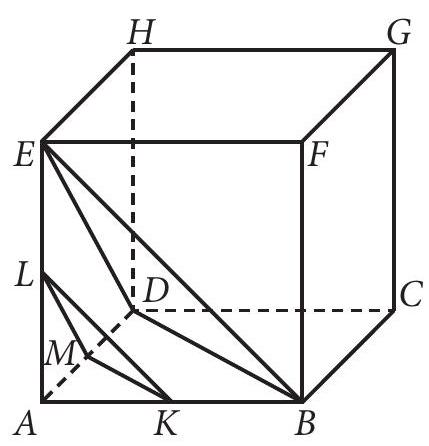
\includegraphics[max width=\textwidth, center]{2024_11_21_dd21f7544b65bcf1b3c7g-20}

Więcej arkuszy znajdziesz na stronie: \href{http://arkusze.pl}{arkusze.pl}

\begin{center}
\begin{tabular}{|c|c|c|c|c|c|c|c|c|c|c|c|c|c|c|c|c|c|c|c|c|c|c|c|c|c|c|c|c|c|}
\hline
 &  &  &  &  &  &  &  &  &  &  &  &  &  &  &  &  &  &  &  &  &  &  &  &  &  &  &  &  &  \\
\hline
 &  &  &  &  &  &  &  &  &  &  &  &  &  &  &  &  &  &  &  &  &  &  &  &  &  &  &  &  &  \\
\hline
 &  &  &  &  &  &  &  &  &  &  &  &  &  &  &  &  &  &  &  &  &  &  &  &  &  &  &  &  &  \\
\hline
 &  &  &  &  &  &  &  &  &  &  &  &  &  &  &  &  &  &  &  &  &  &  &  &  &  &  &  &  &  \\
\hline
 &  &  &  &  &  &  &  &  &  &  &  &  &  &  &  &  &  &  &  &  &  &  &  &  &  &  &  &  &  \\
\hline
 &  &  &  &  &  &  &  &  &  &  &  &  &  &  &  &  &  &  &  &  &  &  &  &  &  &  &  &  &  \\
\hline
 &  &  &  &  &  &  &  &  &  &  &  &  &  &  &  &  &  &  &  &  &  &  &  &  &  &  &  &  &  \\
\hline
 &  &  &  &  &  &  &  &  &  &  &  &  &  &  &  &  &  &  &  &  &  &  &  &  &  &  &  &  &  \\
\hline
 &  &  &  &  &  &  &  &  &  &  &  &  &  &  &  &  &  &  &  &  &  &  &  &  &  &  &  &  &  \\
\hline
 &  &  &  &  &  &  &  &  &  &  &  &  &  &  &  &  &  &  &  &  &  &  &  &  &  &  &  &  &  \\
\hline
 &  &  &  &  &  &  &  &  &  &  &  &  &  &  &  &  &  &  &  &  &  &  &  &  &  &  &  &  &  \\
\hline
 &  &  &  &  &  &  &  &  &  &  &  &  &  &  &  &  &  &  &  &  &  &  &  &  &  &  &  &  &  \\
\hline
 &  &  &  &  &  &  &  &  &  &  &  &  &  &  &  &  &  &  &  &  &  &  &  &  &  &  &  &  &  \\
\hline
 &  &  &  &  &  &  &  &  &  &  &  &  &  &  &  &  &  &  &  &  &  &  &  &  &  &  &  &  &  \\
\hline
 &  &  &  &  &  &  &  &  &  &  &  &  &  &  &  &  &  &  &  &  &  &  &  &  &  &  &  &  &  \\
\hline
 &  &  &  &  &  &  &  &  &  &  &  &  &  &  &  &  &  &  &  &  &  &  &  &  &  &  &  &  &  \\
\hline
 &  &  &  &  &  &  &  &  &  &  &  &  &  &  &  &  &  &  &  &  &  &  &  &  &  &  &  &  &  \\
\hline
 &  &  &  &  &  &  &  &  &  &  &  &  &  &  &  &  &  &  &  &  &  &  &  &  &  &  &  &  &  \\
\hline
 &  &  &  &  &  &  &  &  &  &  &  &  &  &  &  &  &  &  &  &  &  &  &  &  &  &  &  &  &  \\
\hline
 &  &  &  &  &  &  &  &  &  &  &  &  &  &  &  &  &  &  &  &  &  &  &  &  &  &  &  &  &  \\
\hline
 &  &  &  &  &  &  &  &  &  &  &  &  &  &  &  &  &  &  &  &  &  &  &  &  &  &  &  &  &  \\
\hline
 &  &  &  &  &  &  &  &  &  &  &  &  &  &  &  &  &  &  &  &  &  &  &  &  &  &  &  &  &  \\
\hline
 &  &  &  &  &  &  &  &  &  &  &  &  &  &  &  &  &  &  &  &  &  &  &  &  &  &  &  &  &  \\
\hline
 &  &  &  &  &  &  &  &  &  &  &  &  &  &  &  &  &  &  &  &  &  &  &  &  &  &  &  &  &  \\
\hline
 &  &  &  &  &  &  &  &  &  &  &  &  &  &  &  &  &  &  &  &  &  &  &  &  &  &  &  &  &  \\
\hline
 &  &  &  &  &  &  &  &  &  &  &  &  &  &  &  &  &  &  &  &  &  &  &  &  &  &  &  &  &  \\
\hline
 &  &  &  &  &  &  &  &  &  &  &  &  &  &  &  &  &  &  &  &  &  &  &  &  &  &  &  &  &  \\
\hline
 &  &  &  &  &  &  &  &  &  &  &  &  &  &  &  &  &  &  &  &  &  &  &  &  &  &  &  &  &  \\
\hline
 &  &  &  &  &  &  &  &  &  &  &  &  &  &  &  &  &  &  &  &  &  &  &  &  &  &  &  &  &  \\
\hline
 &  &  &  &  &  &  &  &  &  &  &  &  &  &  &  &  &  &  &  &  &  &  &  &  &  &  &  &  &  \\
\hline
 &  &  &  &  &  &  &  &  &  &  &  &  &  &  &  &  &  &  &  &  &  &  &  &  &  &  &  &  &  \\
\hline
 &  &  &  &  &  &  &  &  &  &  &  &  &  &  &  &  &  &  &  &  &  &  &  &  &  &  &  &  &  \\
\hline
\end{tabular}
\end{center}

Więcej arkuszy znajdziesz na stronie: \href{http://arkusze.pl}{arkusze.pl}\\

\includegraphics[max width=\textwidth, center]{2024_11_21_dd21f7544b65bcf1b3c7g-21}

Odpowiedź:

\begin{center}
\begin{tabular}{|l|l|c|}
\hline
\multirow{2}{*}{\begin{tabular}{c}
Wypełnia \\
sprawdzający \\
\end{tabular}} & Nr zadania & 32 \\
\cline { 2 - 3 }
 & Maks. liczba pkt & 5 \\
\cline { 2 - 3 }
 & Uzyskana liczba pkt &  \\
\hline
\end{tabular}
\end{center}

Więcej arkuszy znajdziesz na stronie: \href{http://arkusze.pl}{arkusze.pl}\\

\includegraphics[max width=\textwidth, center]{2024_11_21_dd21f7544b65bcf1b3c7g-22}

\section*{WPISUJE ZDAJĄCY}
\begin{center}
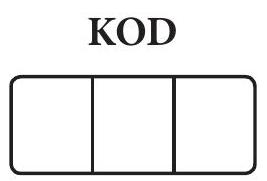
\includegraphics[max width=\textwidth]{2024_11_21_dd21f7544b65bcf1b3c7g-23}
\end{center}

IMIĘ I NAZWISKO *

\begin{itemize}
  \item nieobowiązkowe
\end{itemize}

KARTA ODPOWIEDZI

\begin{center}
\begin{tabular}{|c|c|c|c|c|c|}
\hline
 & \( \mathrm{Nr} \) &  & Odpo & iedzi &  \\
\hline
 & 1 & A & B & C & D \\
\hline
 & 2 & A & B & C & D \\
\hline
 & 3 & A & B & C & D \\
\hline
 & 4 & A & B & C & D \\
\hline
枵 & 5 & A & B & C & D \\
\hline
N & 6 & A & B & C & D \\
\hline
들 & 7 & A & B & C & C \\
\hline
\( \ddot{~} \) & 8 & A & B & C & D \\
\hline
응 & 9 & A & B & C & D \\
\hline
g & 10 & A & B & C & D \\
\hline
N & 11 & A & B & C & D \\
\hline
\( \stackrel{N}{\sim} \) & 12 & A & B & C & D \\
\hline
స్ & 13 & A & B & C & D \\
\hline
ట్চ & 14 & A & B & C & D \\
\hline
并 & 15 & A & B & C & D \\
\hline
'ষ্ & 16 & A & B & C & D \\
\hline
 & 17 & A & B & C & D \\
\hline
 & 18 & A & B & C & D \\
\hline
 & 19 & A & B & C & D \\
\hline
 & 20 & A & B & C & D \\
\hline
 & 21 & A & B & C & D \\
\hline
 & 22 & A & B & C & D \\
\hline
 & 23 & A & B & (C) & D \\
\hline
\end{tabular}
\end{center}

WYPEENIA SPRAWDZAJĄCY

\begin{center}
\begin{tabular}{|c|c|c|c|c|c|c|}
\hline
\multirow{2}{*}{\begin{tabular}{c}
Nr \\
zad. \\
\end{tabular}} & \multicolumn{6}{|c|}{Punkty} \\
\hline
 & \(\mathbf{0}\) & \(\mathbf{1}\) & \(\mathbf{2}\) & \(\mathbf{3}\) & \(\mathbf{4}\) & \(\mathbf{5}\) \\
\hline
\(\mathbf{2 4}\) & \(\square\) & \(\square\) & \(\square\) &  &  &  \\
\hline
\(\mathbf{2 5}\) & \(\square\) & \(\square\) & \(\square\) &  &  &  \\
\hline
\(\mathbf{2 6}\) & \(\square\) & \(\square\) & \(\square\) &  &  &  \\
\hline
\(\mathbf{2 7}\) & \(\square\) & \(\square\) & \(\square\) &  &  &  \\
\hline
\(\mathbf{2 8}\) & \(\square\) & \(\square\) & \(\square\) &  &  &  \\
\hline
\(\mathbf{2 9}\) & \(\square\) & \(\square\) & \(\square\) & \(\square\) &  &  \\
\hline
\(\mathbf{3 0}\) & \(\square\) & \(\square\) & \(\square\) & \(\square\) & \(\square\) &  \\
\hline
\(\mathbf{3 1}\) & \(\square\) & \(\square\) & \(\square\) & \(\square\) & \(\square\) & \(\square\) \\
\hline
\(\mathbf{3 2}\) & \(\square\) & \(\square\) & \(\square\) & \(\square\) & \(\square\) & \(\square\) \\
\hline
\end{tabular}
\end{center}


\end{document}